\documentclass{report}
\usepackage{longtable}
\usepackage{listings}
\usepackage{graphicx}
\usepackage{multirow}
\usepackage{fontspec}
\usepackage[section]{placeins}

\newfontfamily{\ttconsolas}{Consolas}

\title{Lab7\_Finite State Machine design}
\author{201704150 Kangjun Heo}

\lstset{basicstyle=\ttfamily,breaklines=true}
\lstset{framextopmargin=10pt,framexbottommargin=10pt,frame=tb}


\begin{document}
    \maketitle
    \tableofcontents

    \chapter{Purpose of the lab}

        \paragraph{This lab aims to design Finite State Machine in two types - Moore Machine and Mealy Machine - with Verilog language. This report contains state diagrams, waveforms and verilog codes with test cases.}
    
        \section{Finite State Machine}

        \paragraph{\normalfont Finite State Machine is a fundamental mathematical model that describes sequencial logic. There are two types of FSM - Moore Machine and Mealy Machine. Former one defines output with its state, otherwise, latter one defines output not only with its state, but includes current input.}

        \section{Requirements of Target Machine}

        \paragraph{\normalfont Desired finite state machine can output 0 until same inputs received after 4 positive clock edge. otherwiese, output 1.}
    \chapter{Design Procedure}

        \begin{figure}[!htb]
            \centering
            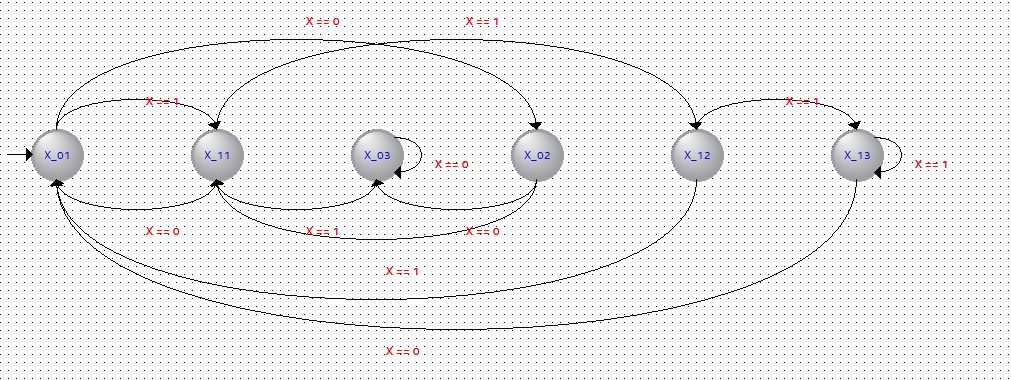
\includegraphics[width=\textwidth]{diagrams/mealy_statediagram.PNG}
            \caption{State Diagram of Desired Mealy Machine}
        \end{figure}

        \begin{figure}[!htb]
            \centering
            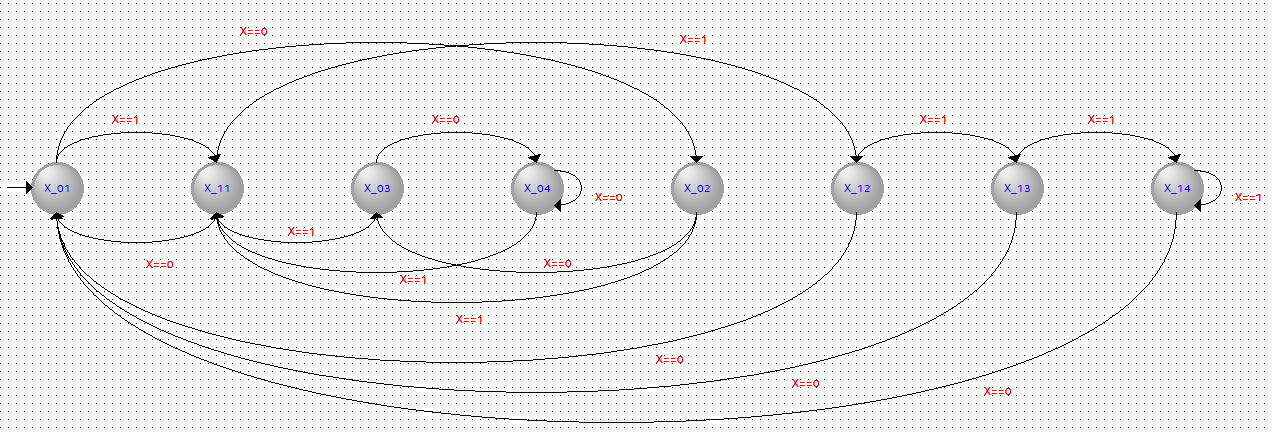
\includegraphics[width=\textwidth]{diagrams/moore_statediagram.PNG}
            \caption{State Diagram of Desired Moore Machine}
        \end{figure}

    \chapter{Simulation}
        \section{Source Code}
            \lstinputlisting[caption=Top Module]{fsm/fsm_top.v}
            \lstinputlisting[caption=Mealy Machine]{fsm/fsm_mealy.v}
            \lstinputlisting[caption=Moore Machine]{fsm/fsm_moore.v}
        \section{Testbench}
            \begin{figure}[!htb]
                \centering
                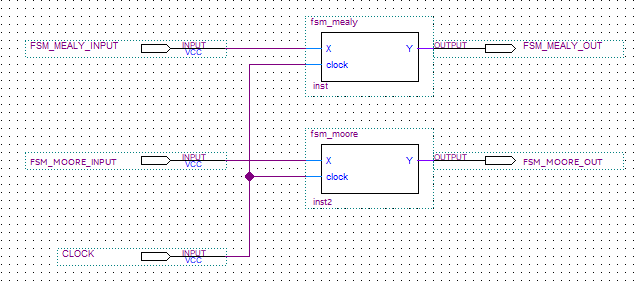
\includegraphics[width=\textwidth]{diagrams/block_diagram.PNG}
                \caption {Block diagram of Testbench}
                \label{fig:wf-0}
            \end{figure}
            \lstinputlisting[caption=Testbench Code]{fsm/fsm_tb.v}

        \section{Simulation Result}
            \begin{figure}[!htb]
                \centering
                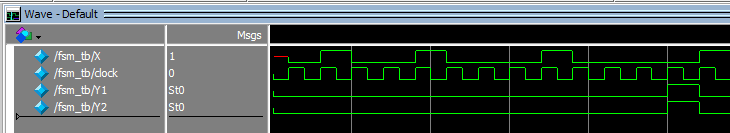
\includegraphics[width=\textwidth]{diagrams/waveform-first.png}
                \caption {First Result Set of Simulation}
                \label{fig:wf-1}
            \end{figure}

            \begin{figure}[!htb]
                \centering
                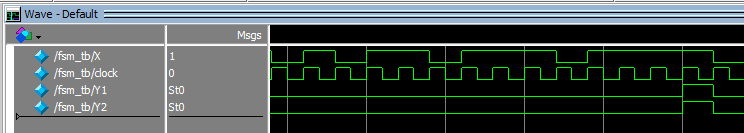
\includegraphics[width=\textwidth]{diagrams/waveform-second.png}
                \caption {Second Result Set of Simulation}
                \label{fig:wf-2}
            \end{figure}

            \begin{figure}[!htb]
                \centering
                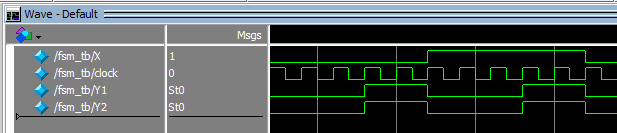
\includegraphics[width=\textwidth]{diagrams/waveform-last.png}
                \caption {Last Result Set of Simulation}
                \label{fig:wf-3}
            \end{figure}

    \chapter{Evaluation}
        \paragraph{\normalfont According to Figure~\ref{fig:wf-1}, Figure~\ref{fig:wf-2}, Figure~\ref{fig:wf-3}, for each test cases, proper waveforms are generated. Both of two machines, their waveforms were identical.}  

    \chapter{Discussions}
        \section{Key Part of This Lab}
            \paragraph{\normalfont The output of sequencial logic is not determined only by current input, but also previous inputs that is so-called "state". Any of specific module is controlled by "clock" which oscillates between 0 and 1 at constant interval. This FSM gets input and changes state or output when clock reaches positive edge. At this point, Moore Machine determines its state with input, but output is determined by its state only. However, Once Mealy Machine receives positive clock edge, it gets input, determines output with state and input, then makes its state transition. Thanks to this aspect of Mealy Machine, lesser states can be defined when its design while maintaining its functionality.}

        \section{Mistakes}
            \paragraph{\normalfont Verilog supports C-like condition expression. Initial version of Mealy Machine didn't generate proper waveform - its output was statically 0 - also its states were not changing as if they were not affected by the input. As I figured out, \texttt{!=} operator didn't work as expectation. Therefore the condition was flipped, then the waveform was generated in proper form.  }

        \section{Expected Improvements}
            \paragraph{\normalfont Conditional branches are useful when designing modules in behavior form. However, Its mechanism is not exactly same as other C-like languages so different plotting is required when using it.}
\end{document}